%
% File: chap01.tex
% Author: Victor F. Brena-Medina
% Description: Introduction chapter where the biology goes.
%
\let\textcircled=\pgftextcircled
\chapter{Introduction}
\label{chap:intro}

\initial{E}nergy is the bashape of not only our modern society, but is also the source of all transformations that lead us here, from the control and use of fire for tools to the coal that powered the start of the industrial revolution and  the electricity that runs most households across the world nowadays. 

According to the World Energy Council (2015), 1.2 billion people do not  have access to electricity. Accentuating the situation, the energy price volatility also reported and the greenhouse gas emissions issue point out a need for cheap, reliable and renewable energies.  Despite its availability, some renewable resources, such as tidal and wave energy are not yet a reality and might play an important role in the future. Being able to improve power take-off technologies play an important role to make renewable energies feasible.
On the other hand, the popularization of electronics and their dependence on batteries also rises as a technical issue (as more powerful devices are limited by their autonomy) and environmental issue, as batteries cannot be disposed trivially.
Being able to perform in both those situations described, Dielectric Elastomer Generators (DEGs) should play an important role in future. Although more established technologies such as electromagnetic generators, are strong competitors, DEGs have a great potential, as shown in Table 1. Their high energy density, allied with low raw materials’ prices provide great advantage when compared to other technologies.
\paragraph{} According to the World Energy Council\cite{EnergyIssues}, 1.2 billion people do not have access to electricity. Energy price volatility and greenhouse gas emissions issue accentuate this issue, and point to the need for cheap, reliable and renewable energies.  As a new and emerging eletromechanical energy conversion technology, Dielectric Elastomer Generators (DEGs) are one possible solution. With low frequency and wide bandwidth\cite{Boots2buoys}, energy harvesting DEGs have already been reported for use in wave energy generation \cite{VertechyPolyWECtest2014}, human motion energy harvesting\cite{MistralHMotion2008} and even as thermal machines\cite{Boots2buoys}.
\paragraph{} DEGs harvest energy through capacitance change induced by  deformation. The energy harvesting happens in cycles; one example with four stages I--IV is illustrated in Figure \ref{fig:cycle}. The transitions between states in this cycle are as follows.
\begin{itemize}
\item I$\rightarrow$II: From an initially relaxed phase, the DEG is stretched by a mechanical load and increases its capacitance.
\item II$\rightarrow$III: Once stretched, the DEG is polarized through an electrical energy input.
\item III$\rightarrow$IV: From stretched and polarized, in an open circuit configuration, the mechanical load is released letting the material relax, so reducing the DEG's capacitance. As the capacitance reduces and the charge stored is maintained constant, there is a voltage rise.
\item IV$\rightarrow$I: Finally, the DEG is discharged from its more energetic state, back to its initial state.
\end{itemize}

% \begin{figure}[ht]
% \begin{center}
% \begin{tabular}{c}
% 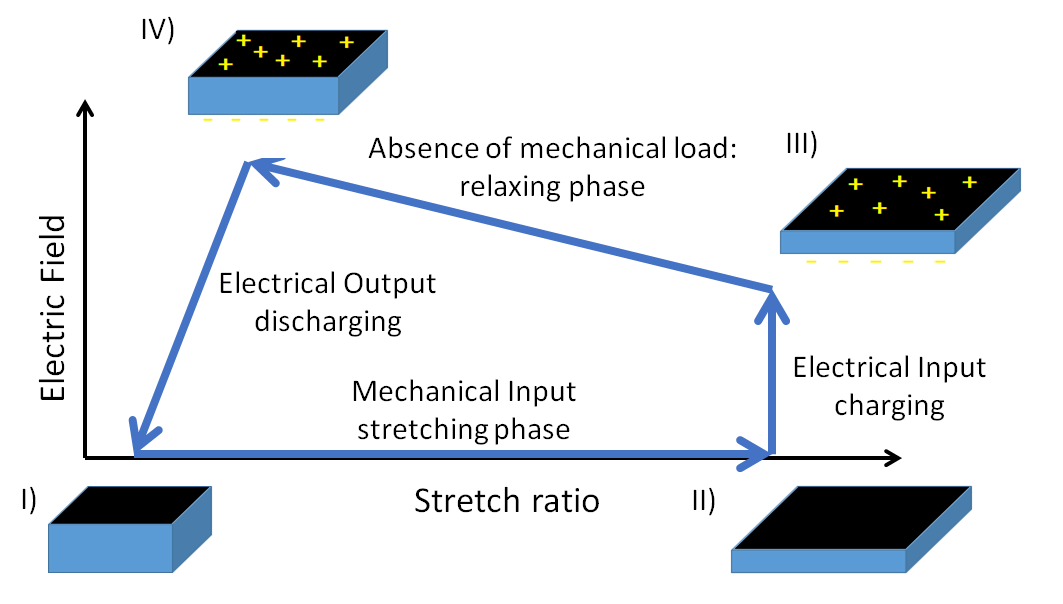
\includegraphics[height=6cm]{fig03/Cycle.png}
% \end{tabular}
% \end{center}
% \caption 
% { \label{fig:cycle}
% DEG energy harvesting cycle using relaxation with constant charge} 
% \end{figure} 

\paragraph{} Among the drawbacks of current DEG technology is the necessary condition of inputting electrical energy to polarize the material. Furthermore, the energy output between states IV and I is proportional to the amount of electrical energy used to polarize the DEG between states II and III\cite{DEGCycles}, so, in order to explore the energy harvesting capabilities at its maximum, one might want to input high voltages.

Table 1. Comparison of dielectric elastomer with other power generation technologies. Adapted from (Kornbluh et al., 2012).
Technology	Energy Density (J/g)	Conversion Efficiency	Comment
Dielectric elastomer	0.4 (.05 for long lifetime operation)	>50%	Low-cost non-toxic materials, low stiffness, size scalable

Electromagnetic	0.004	<20\%	Low-energy density, constant-frequency electromagnetic generators can have much higher efficiency, but need variable frequency transmission for higher efficiency over a range of frequencies

Piezoelectric ceramic	0.01	>50\%	Requires significant additional mass for support or motion amplification, expensive (and often toxic) materials

Despite the potential advantages, dielectric elastomer generators are still not a reality and commercial applications are still under development. Dielectric Elastomers (DEs) are smart materials that can be explored in several ways: actuators, generators and are also able to modify their stiffness. Due to their novelty, there are still gaps on the knowledge of their behaviour and physics that should be better explored.   The present work seeks to understand how all these different behaviours (actuator, generator and stiffness controller) can be synchronized to   provide better energy harvesting capabilities. 
The present report is organised in an initial chapter that describes and evaluates literature on DEGs, describing work performed previously and that provide the basis of knowledge for the current project. The following chapter presents the work we have done on cycle modelling and suggests how the generators behaviour could be enhanced.  Next, we describe the models developed to support our research and finally present one parallel investigation on self-priming circuits, which present a good alternative for the high voltage supply issue characteristic of DEGs. The report is concluded by an outline of future work for the next months.
In the appendix can be found a report about courses and events attended, the mathematical deduction of the model presented about self-priming circuits, the abstract submitted to EAPAD 2016 and the paper submitted to Applied Physics Letters. 
Dielectric Elastomer Generators – Overview

We begin by presenting the concept of Dielectric Elastomer Generators (DEGs), dielectric elastomers (DEs) used to convert mechanical to electrical energy, which are the central focus of the present project. Through definitions and examples from literature, the operating principles of DEGs will be explained, in order to provide an understanding of the activities that will be reported on the following chapters.
Dielectric Elastomers and their actuator mode

 
Figure 1. Dielectric Elastomer basic configuration. From Tepel et al. (2013)
DEs are a class of smart materials inside the group of electroactive polymers, those that react to electric stimulation. DEs consist of a highly flexible insulator membrane coated with flexible conductive layers. This creates a flexible capacitor-like structure, where the membrane in the middle isolates the charges on the conductive layers, the electrodes (see scheme in Figure 1). DEs were initially explored as actuators, transducing the electrical stimulation into mechanical response (Pelrine et al., 2000). Their working principle is based on the electrostatic stress, which is commonly referred to as Maxwell Stresses. Maxwell Stresses are generated normal to the film’s plane by the induced electric field when there are charges on the electrodes. The electrostatic force compresses the insulator film producing a deformation in the plane of the film. The electrostatic force works against the elastic forces, accumulating part of the electric potential energy as elastic energy. This principle explains the actuator mode, when electrical energy is converted into mechanical energy.  Figure 2 illustrates the process and provides an example of the process.
 
Figure 2. Dielectric elastomer actuators. a)Working principle. From Carpi et al. (2008). b)Example of circular actuator assembled on a frame. From Pelrine et al. (2000).
The literature has suggested that DEs are a promising technology, as they are characterised by high actuation speed, low cost, high strain, high energy densities and efficiencies (Pelrine et al., 1998, Pelrine et al., 2000). This gives them an advantage, on a small-scale actuation,  when compared to other technologies, such as shape memory alloys, electromagnetic micro actuators and piezoelectric actuators (Pelrine et al., 2000). 

Dielectric Elastomer Generators

DEs can also be used to convert mechanical to electrical energy. Once DEs are stretched, if charged and allowed to relax, the elastic forces will work against the electrostatic forces created by the Maxwell Stress, moving the opposite charges apart and pushing like charges closer due to the electrode area reduction. This process leads to an electrostatic potential increase.
In contrast with piezo ceramics and other polarized materials, DEs do not have natural polarization, needing an external electrical stimulus prior to this relaxing process in order to yield any energy conversion.  A typical energy conversion cycle is shown in Figure 3: The material is initially stretched by external mechanical forces from a free of charges state (A) to a still free of charge state (B). From state B, it is charged with an initial priming voltage (C) receiving an initial electric energy input. From state C, still deformed, the material is allowed to relax to a higher electrical energy state (D). From state D, it outputs the electrical energy stored and returns to the initial state (A).
 
Figure 3. Electrical to mechanical energy converting cycle.
	The following sections will cover details about the energy conversion cycles, adequate materials, performance capabilities and possible applications of DEGs.

Mechanical to electrical energy converting cycles

	Several studies, described in more detail below, have focused on optimizing the energy conversion cycle, looking for improvements in energy harvested per cycle, loss reduction, efficiency increase, among other goals. 
A simple approach that explains the basics of the energy harvesting cycle design is that of Graf et al. (2010b). The authors consider three different possibilities regarding the electrical loads on the relaxing phase: constant charge, constant voltage and constant electric field (see Figure 4). The cycles designed consider the stretch bounded between two levels of strain and the electric field is limited by the Dielectric breakdown (DBS), DEG’s most known failure, when the insulator becomes conductive and allows current to pass.
Constant charge is the simplest case, when electrical energy is loaded between states 2 and 3, discharged between states 3 and 4 and there is no electric current while the DEG relax (phase 3-4), when the circuit is left open. Constant voltage cycles differ as the DEG remains connected to a constant voltage source during the relaxing phase; as a result part of the energy gain is drained during this phase. The constant electric field cycle takes advantage of the fact that the maximum energy harvested per cycle will be achieved when cycle area is maximum. Hence, it uses a really high energy input and relies on a control system to drain the energy gain during the stretch phase avoiding the electric field increase that could lead to dielectric breakdown (hypothesised as constant for their model). 
To quantify the performance of a DEG, we compute the electrical energy harvested as the difference between the electric energy input (used to polarize the material) and the electrical energy output (the energy discharged):
%	Ue_harv=Ue_out-Ue_in.	( 1 )

Graf et al. (2010b) compared the performance of each cycle as a function of the stretching applied $(α=(Area_min)/(Area_max )) $ using the amount of energy harvested per cycle and the relative energy gain (energy harvested per unit of energy used to polarize) as performance metrics. Figure 5 shows that both metrics increase as the stretching increases. Constant charge cycles present the best relative energy gain, while constant field present the highest amount of energy harvested per cycle. Moreover, these different cycles were conducted experimentally by Dimopoulos et al. (2012). The authors reported the advantage on easier pre-selection of electronic components on the constant voltage cycle, since maximum voltage can be known prior to the implementation.
	Still using a perspective based on these cycles, studies have evaluated the electric losses induced: in the electrodes, through leakage, and due to the power electronics. They have been modelled as functions of the stretch, charge input and cycle relaxing phase process (Graf et al., 2014, Graf et al., 2010b, Graf et al., 2010c). In a more general line of attack, the losses in the DEG can be split in two: the charge leakage (current that flows through the insulator) and the energy dissipated in the electrodes. The former is usually modelled as a parallel resistor and represents an important issue, especially for low frequency cycles, when the DEG is subjected to a high voltage for a higher amount of time(Graf et al., 2010b). Losses in the electrodes are usually represented by a resistor in series and can have a strong dependence on the stretch, since it will affect the electrode shape (thickness and area). Both can be modelled as stretch dependent and this method should be used when the stretch levels investigated increase(Graf et al., 2010c). Figure 6 illustrates the electric model.
 
Figure 6. Electric model of DEG including losses. Rp represent the polymer resistance and Re the electrodes resistance
	Several studies have been carried out in order to determine optimized parameters for the energy harvesting cycle and even to optimize its “shape” combining parts of the basic ones listed above (Ahnert et al., 2011, Dimopoulos et al., 2012, Hoffstadt et al., 2013, Koh et al., 2011, Koh et al., 2009, Shian et al., 2014, van Kessel et al., 2010, Wang et al., 2012). Fundamentally, the cycle optimizations seek to increase energy conversion efficiency, energy gain per cycle or relative energy gain while avoiding the material failures modes. Koh et al. (2009)  used the Neo-Hookean material model and determined the cycle boundaries through the modes of failure. Figure 7 illustrates the cycle design by an example of cycle that mixes constant charge and constant voltage. Although cycles designed using such limits, should be, theoretically, able to maximise the energy conversion, there is still flexibility on how to position the states and the losses to be considered.
		Most cycle modifications and adaptations tend to seek a higher energy conversion, but the charging phase, when most of the losses happen, also requests some attention. Wang et al. (2012) tested the idea of charging while stretching, since it should reduce the losses caused by high current when charging on a short time span. The authors demonstrated that this process change could be advantageous, since the energy conversion decrease (due to the internal area of the cycle being reduced) is inferior to the charging losses reduction. Despite their interesting experimental findings, there is a lack of theoretical support to understand better the process, and look for improvements.
	Another relevant point to be made about the energy harvesting cycle regards how the states are modelled. Graf et al. (2014) split it into 3 cases:
	Position based: DEG stretch alternates between two different positions only. In practice, corresponds to cases where mechanisms such as crank and slider are used.
	Force based: DEG stretch is based on an alternating force, switching between two states and kept constant during charge and discharge. This could be used to represent wave energy cases, when the DEG stretch is not mechanically limited, given that the charging and discharging are fast enough for the mechanical load to be considered constant during them.
	The third case is a more realistic version of the force-based cycle, when the force is not kept constant during charge and discharge and accounts for the dynamic effects that should be included.



Modelling and performance prediction

	DEs are no trivial material to be modelled. Their nonlinear mechanical behaviour challenges the task of obtaining simple analytical models, restraining simple Hookean models to low stretch cases and limiting their performance simulation mostly to numerical models. 
 
Figure 8. Different material models fit for a rubber-like material such as those used in DEGs. From Kofod (2001).
	In order to simulate the mechanical behaviour of DEs, many hyperelastic material models have been used to model DEs, such as the Neo-Hookean (Hackl et al., 2005, Graf et al., 2010a, Zhao et al., 2007), Yeoh (Ahnert et al., 2011, Wissler and Mazza, 2005a, Wissler and Mazza, 2007a, Wissler and Mazza, 2005b), Ogden (Wissler and Mazza, 2005b, Wissler and Mazza, 2007a), Mooney-Rivlin (Binh et al., 2015, Jean-Mistral et al., 2010), Arruda-Boyce (Koh et al., 2011, Zhao et al., 2007) and Gent (Foo et al., 2012, Huang and Suo, 2012). Figure 8 shows characteristic curves for some of them. Although more limited in its accuracy, the Neo-Hookean model is the most straightforward for crude analytical modelling, since it can be described using only the material’s shear modulus (G). It has been the model used in my research so far.
	In the Neo-Hookean model, the strain energy for an incompressible material is given by
$	W_(〖strain〗_NeoHookean )=G(I_1-3)/2,$
( 2 )
where $I_1$ is the first invariant of the Cauchy-Green deformation tensor and is itself given by the stretch ratios %λ_x, λ_y and λ_z in the three coordinate directions:
%	I_1= 〖λ_x〗^2+〖λ_y〗^2+〖λ_z〗^2.
( 3 )
The electromechanical coupling, $σ_Maxwell$, is given by the Maxwell Stress equation,
%	σ_Maxwell= e_r e_0 E^2,
( 4 )
a function of the dielectric permittivity of vacuum ($e_0$), dielectric permittivity of the insulator ($e_r$) and the electric field applied ($E$)(Carpi et al., 2008).
Considering the necessary boundary conditions, the electromechanical coupling and using a Neo-Hookean model, it is possible to obtain equations to describe the DEG states in biaxial stretch, pure shear conditions and uniaxial stretch. From (Graf et al., 2010a), the equation to model a pure shear case (uniaxial stretch with constant material width, see Figure 9) is given by:
%	m(x ) ̈=F_x- d_v x ̇-  B/x (G (〖λ_x〗^4-1)/〖λ_x〗^2 +σ_z ),
( 5 )
where m is the equivalent mass, $F_x$ is the applied force, $d_v$ is the damping coefficient and $B$ is the total volume of the DEG. The applied stress, $σ_z$, is given by 
%	σ_z=-σ_Maxwell.
( 6 )
Also from (Graf et al., 2010a), for a biaxial stretch the model can be described by 
%	m(x ) ̈=F_x- d_v x ̇-  B/x (G (〖λ_x〗^6-1)/〖λ_x〗^4 +σ_z ),
( 7 )
which allows a fast switch between models once one of them is implemented.
After exploring modelling possibilities and choosing the most adequate one, it is possible to perform optimizations and evaluate how to quantify and how to optimize the performance of DEGs.  Kang et al. (2011) used a simplified linear elastic model to derive an equation for the efficiency of a DEG diaphragm shaped under a constant charge cycle. They concluded that the DEG efficiency is inversely proportional to the material stiffness, proportional to the dielectric permittivity, which is the number of layers the square of the bias voltage. For the case hey considered, the DEG efficiency (electric energy harvested per amount of mechanical energy used to stretch the DEG) is reported around 2\%-3\% for a bias voltage of 1kV. In Kaltseis et al. (2011), a method to measure the DEG efficiency experimentally demonstrated efficiency of 7.5\% (considering the electric energy harvested per amount of mechanical energy absorbed) on a cycle that mixed constant charge followed by voltage, with input voltage of 2.5kV.

Materials

	From the initial studies with DEs, the most used materials for actuators and generators have been silicones and acrylic, particularly 3M tape VHB, since they present low stiffness and high stretch capabilities. VHB has reported energy density as high as 0.4J/g (Pelrine et al., 2001), although the experimental conditions were not specified and contrast with most other findings around 10-100mJ/g (Kaltseis et al., 2011, Wang et al., 2012, Mckay et al., 2010a). Koh et al. (2011) calculated that the maximum energy that could be converted by VHB is 1.7J/g evaluating through the limits of material failure. Despite its high stretching and low stiffness, which allows VHB to be a good candidate for DEGs, VHB is a highly viscous material. Indeed, these viscous losses compromise its overall energy conversion, especially on high frequencies, when a great part of the mechanical input is dissipated instead of stored as elastic energy. 
Silicones are still popular, but few studies report experimental values for their energy density and the wide variety of popular formulations make comparisons even harder. Pelrine et al. (2001) reported that energy densities of 13mJ/g were achieved, but estimated that it could go as high as 1J/g. Silicones were also explored to produce interpenetrating polymer networks (IPN) (Yu et al., 2015), which aim to combine high permittivity without compromising materials flexibility and dielectric breakdown limit. 
Another possible material is natural rubber. Kaltseis et al. (2014) used the same procedure as Koh et al. (2011) and obtained that, for two natural rubber types, the energy density could be as high as 3.0J/g and 3.5J/g. Using an experimental approach to observe the viability of natural rubber, the authors achieved energy harvesting levels up to 210mW/g, with 14.9\% of mechanical-to-electrical energy conversion. They used an inflated DEG diaphragm, as described in (Kaltseis et al., 2011) for VHB (there yielding 102mJ/g). Despite being stiffer and having lower stretching capabilities, natural rubber seems a promising material as it is not as viscous as VHB and has a higher dielectric breakdown voltage (see Figure 10). 
	Taking into account its higher dielectric permittivity (from 6 to 8) and dielectric breakdown voltages (over 100MV/m), studies with polyurethane look promising (Graf et al., 2014). On a comparative study, Graf et al. (2014) reported energy gain of 5.43J/cm3 in a polyurethane formulation versus 1.79J/cm3 of their formula of silicone under same conditions. As in silicones, the variety of formulations and the lack of detail on manufacturing processes in reported work create a complicated base for comparative future work.
	Although several performance numbers could be collected from literature, fair comparisons are hardly ever possible, since several factors affect it, from bias voltage and cycle to electrode choice. Moreover, most of the reported experiments aim for reporting a new concept, not necessarily using the optimum conditions for energy density of other performance metric.
	With regard to the electrodes, it has also already been demonstrated that they have a major influence as they play a major role in the electrical losses. Due to its easy application allowing fast DEG fabrication, carbon grease has been a popular choice(Mckay et al., 2010a, Kaltseis et al., 2011, Kang et al., 2011), but studies with metallic electrodes have also been conducted (Carpi et al., 2008). 

DEG setup enhancement

		While materials and the optimal cycles for energy harvesting are topics of research by themselves, other ways to improve DEG efficiency, or broaden their application boundaries are also being explored. Mapping DEGs’ energy gains, losses and conversions are an important starting point to understand where the biggest possibilities of improvement are. Figure 11 outlines the energy conversions and processes through the energy harvesting process. 
Figure 11. Energy flow and conversion through the DEG energy mechanical to electrical energy transducing process.
Intuitively, once acknowledging that part of the mechanical energy inputted to the system to generate the stretch is also outputted as the material relaxes, an antagonistic system is a natural idea to be explored. A comparative study of a system with a single DEG against an antagonistic pair of DEGs was made by Binh et al. (2014) and showed that it could improve the amount of mechanical energy absorbed by 150\% and raise the overall efficiency from 7.61% to 17.19%. Although its potential application was outlined as wave energy converters, its implementation is not clear. Indeed, the test conditions used uniaxial stretching driven by a slider-crank mechanism that bounds the stretching to a position based cycle, which does not emulate its real world application. 
 	Another point of improvement that can be noticed when observing the energy flow regards the electric energy input needed. Noticing the need for priming at every cycle and that the energy harvested is proportional to it, an important point was made by Mckay et al. (2010b). A self-priming circuit (SPC) was developed, which would passively store part of the electrical energy output and prime it back as energy input on the following cycle, thus permitting a voltage increase at each cycle. The SPC is based on an arrangement of diodes and capacitors that, according to the DEG voltage level, would toggle between a higher and a lower capacitance. Design rules for the SPC were later published (McKay et al., 2012a) for a generalised case and demonstrated through a system that would prime a solar array provided input (30V) to 1500V. 
	Coupling the idea of a SPC with a generator that could also explore the advantages of an antagonistic system, the opposing DEGs could be explored as capacitors, providing a system able to self-prime without an external capacitor bank (Mckay et al., 2010a), as described in Figure 12. An additional improvement was provided by the development of Dielectric Elastomer Switches (DES) (McKay et al., 2011), consisting of piezoresistive electrodes, fabricated directly onto the stretchable dielectric elastomer membrane, that would have a resistance change when deformed. DES acting as diodes create a fully integrated generator, a single device independent of external electronics to operate, as the electronic components are incorporated. These studies regarding SPC were done mostly using high level simulation tools, such as Simulink and FEA, without a deep analytical point of view. Such approach leads to mostly intuitive design rules and there is still room for further studies on the topic.
	A different setup to improve the charging and creating a passive energy harvester was designed by Vu-Cong et al. (2013). The authors used electrets, which are solid dielectrics with a quasi-permanent electric potential. Using electrets associated with the DEs eliminated the need of a bias voltage for charging at every cycle. Although the idea by itself looks promising, limitations like the rigidity of electrets create design barriers. To overcome this issue, the electret-DE system was designed to allow the electret to fold through a hinge-like structure while the DE stretches and relaxes (see Figure 13). However, this requires the DEG to have a previously known deformation since the electret cannot go over its design capabilities.

DEG Applications

Since DEGs need a cyclic process to convert mechanical-to-electrical energy, their application on renewable energies has, for a long time, been motivated by wave energy converters. Being a not yet popular energy source, DEGs appear as a suitable candidate to make it a reality. Extensive work using buoy prototypes has been done showing promising results and interesting large scale designs (Chiba et al., 2008, Chiba et al., 2013, Masuda et al., 2013). During tank tests of a small scale buoy prototype (Chiba et al., 2013) using constant voltage cycles, power generation of around 35mW was obtained and conversion efficiency from wave energy to electrical energy ranged between 2\% and 7\% (set up and results highlighted in Figure 14). Although oscillation frequency has hardly been explored on DEG, results showed a peak of energy harvested for periods of 1.2s. Figure 14 shows the test layout and results. Since the tests used constant voltage cycles, it is clear that the output could have been higher with an optimal cycle, showing even better results. Regarding materials, the device was only identified as an EPAM (Electroactive Polymer Artificial Muscle), it is hard to compare and hypothesise about improvements regarding this field. One issue regards its application on places where tides have great changes. As the water level changes, the dynamics of the designed system would have to be adjusted, and this issue has not yet being tackled. 

 


Still on wave energy converters, another design being tested and currently developed is the oscillating-water-column wave-energy-converted (Vertechy et al., 2013, Vertechy et al., 2014). The design seems promising, exploiting the diaphragm layout, where great results have been already obtained. Figure 16 outlines the functioning of the device. It is part of a consortium to make DEG in wave energy a reality, PolyWEC, and the combined effort of several institutions combining materials, wave energy and dielectric elastomers expertise brings some expectations over its future. Among the interesting characteristics of this design is the deformation in two different directions, as the pressure goes positive and negative, thus having two DEG cycles for each wave period. Again, questions regarding tidal effect arise, also with regard to whether this could affect positively or negatively in case of a single stroke with double the pressure per wave period. Test results on a 1:50 scale prototype with 90mm of radius obtained 76.9mW for 4cm high waves. In a real world implementation average power of 68kW is expected (Vertechy et al., 2014) when subjected to 2m waves, comparable to the power of a 17m diameter wind turbine on 15m/s winds (Spectrum Energy Systems, 2013) and potentially cheaper.
Another popular source of energy for DEG application is human motion. Ever since the heel-strike energy harvester (Kornbluh et al., 2011, Pelrine et al., 2001), it has always been an important theme. With regards to the shoe experiment, in this case, the heel-strike absorber was composed by a diaphragm like structure connected to a chamber filled with gel, as shown in Figure 16. With every heel strike, the compression would increase chamber pressure and deform the DEGs. The heel-strike generator yielded as much as 1W using 33\% efficiency (Kornbluh et al., 2011). One important point is that it was composed of stacked DEGs, therefore having a multiplier effect on overall harvesting. Jean-Mistral et al. (2008), acknowledging that a shoe generator could be too far from possible devices that would use its power, designed instead a structure to be attached behind the knee, so that it would stretch at every step. Due to safety concerns, the device used lower voltages, 170V, at which 1mW was generated. An important issue when developing human motion energy harvesters, which has not been properly verified on reported studies, is user comfort, especially if scaling up the design for a multilayer stack, when elastic forces could disturb user motion, for example. 
In order to harvest wind energy, experiments using a crank-slider mechanism to convert a turbine rotational movement to a uniaxial stretch of the DEG were conducted (Lin and Wang, 2014, Lin et al., 2011). In (Lin and Wang, 2014), a variation of the crank radius was performed, obtaining the result that higher deformations induced would allow greater energy harvesting, in accordance with what is common knowledge in the area. The lack of data about wind speed, turbine parameters and overall system efficiency does not allow a proper evaluation of DEGs suitability for this kind of application. Another important point is that commercially available electromagnetic energy generators achieve very high efficiency, which has not yet been paired by DEGs. Thus, it is hard to think that a system that converts rotational movement to linear, for DEGs’ use, could be a suitable option for wind energy harvesting.
Generating energy using DEGs as transducers for fluidic flow has been an issue, since DEG’s nature demands cyclic behaviour. Devices using crank-slider mechanisms have been reported for both wind (as shown above) and hydropower. Chiba et al. (2008) showed a waterwheel of 30cm diameter that could harvest 35mJ per revolution, but also did not report enough data to allow efficiency and scalability evaluations. Maas and Graf (2012) reported a concept of flow energy converter that would use a valve actively opening and closing fast enough to create the action of a shock wave to be explored. Although it is definitely a new concept and its investigation is valid, there is no experimental data reported to allow conclusions, and several issues remain to be verified, such as the ratio between harvested energy and that spent to actuate the valve. Another possibility for flow harvesting is exploring the energy from induced vortexes. Hoffstadt et al. (2014) studied a concept of cylinder attached to a rigid structure by DEGs, which, through wind induced turbulence, would vibrate and stretch the DEGs. Figure 17 explains the procedure to generate the cyclic behaviour from the continuous flow. Again, it is a concept to be evaluated, as the paper reports mostly the modelling and an experimental approach that considers only an elastomer without charge (proving the vibration induced deformation idea).
 
Figure 18. a) Vortex induced vibration energy harvesting concept by Hoffstad et al. (2014).  Horizontal layout. b) Vertical layout variation. From Hoffstadt et al. (2014). c) Bladeless wind turbine that uses vortex induced vibrations for energy harvesting (MIT Technology Review, 2015). This concept uses electromagnetic transducers claimed to have 70\% efficiency.
     	Since DEGs work on cycles, another possibility of application is thermal machines, where cyclic processes are used to convert heat to mechanical energy. Thus, DEGs could be incorporated to directly transduce the mechanical movement, usually linear, to electrical energy. Studies using DEGs as chambers for internal combustion engines showed interesting concepts and apparently promising results (Kornbluh et al., 2011), but no paper was published with details, therefore remaining an interesting concept to be investigated.  McKay et al. (2014) experimented to substitute the power piston of a Stirling engine by a DEG and used a voice coil actuator to move the displacer piston. Figure 19 illustrates the design used. Through testing different temperatures and different DEG dimensions, they investigated the electrical energy output, being able to harvest energy from temperature differences as low as 19.5K, which are promising results for low grade heat applications. On the other hand, the energy input required by the voice coil actuator was not measured and it was probably higher than the DEG output, showing the design would require another solution to be implemented. 
Conclusion

DEGs present an important technology to be considered for energy transducing.  Despite the high efficiency on the energy transducing of the material, the whole cycle present losses, such as electrical during charging and discharging, that reduce the DEG overall efficiency. Several cycles have been designed to optimize it and the criteria for selecting among them will depend on several factors, such as the application desired. Despite that, most of them focus on theoretical optimal energy harvesting and aligning factors such as charging/discharging and the losses are still a topic that could be explored. The literature already present plenty of models for DEGs and it allows an easy implementation for most common applications. Although not in the scope of the present project, materials research should be observed as the new materials shall help improve performance and even make DEGs feasible and reliable.  Several set ups were developed and they certainly inspire applications that will be outlined in the present project.


%=========================================================